\begin{frame}{3 L'apprentissage non-suppervisé}
  \begin{itemize}
  \item Données non \textit{labélisées}
  \item La machine apprend par elle même à indentifier une structure
  \item Évaluation des performances compliqué.
  \item Problèmes de classification, réduction de dimensions
  \item \textit{K-means}, \textit{Mean Shift}, \textit{Gaussian Mixture Model}
  \item Analyse en Composante Principale
  \end{itemize}  
\end{frame}

\begin{frame}{3.1 Les algorithmes de clustering}
  \begin{itemize}
  \item \textit{Clustering}: Se rapproche d'un problème de classification (sans labels)
  \item Ces algorithmes cherchent à rassembler les exemples en cluster
  \item À la différence des arbres de décision, le choix du cluster ne s'effectue pas par une suite de décisions simple, mais en déterminant la plus petite distance possible dans l'espace des variables
  \item Utilisés pour la segmentation d'utilisateurs/marchés dans le commerce en ligne mais aussi en génétique
  \item Il faut (dans la majorité des cas) définir au préalable le nombre de clusters à construire (hyperparamètre du modèle)
  \end{itemize}
\end{frame}

\begin{frame}{3.1 K-means}
  \begin{itemize}
  \item Sépare les données en $K$ clusters $C$ d'égale variance (dispersion)
  \item Soit les \textit{centroïdes}, la moyenne des échantillons dans chaque cluster
  \item \textit{K-means} modifie la position des \textit{centroïdes} jusqu'à trouver la valeur qui minimise l'écart moyens des échantillons vis-à-vis de son cluster correspondant
  \item Critère de minimisation: \textbf{inertie}: $I = \displaystyle\sum_{k=0}^{K}\displaystyle\sum_{x \in C_{k}} || x - \mu_{k} ||^{2}$
  \item La performance du \textit{K-means} est fortement dépendante de son initialisation \textit{(Solution: plusieurs initialisation $\rightarrow$ moyenne)}
  \item Le \textit{K-means} ne fonctionne pas avec des variables catégorielles (il existe des adaptations). Il est préférable de normaliser les variables.
  \end{itemize}
\end{frame}

\begin{frame}{3.1 Clustering: Iris dataset, K-means result}
  \begin{figure}
    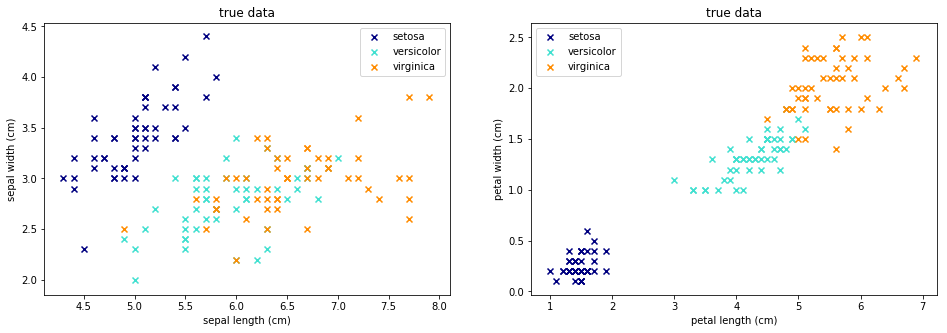
\includegraphics[width=0.9\textwidth]{fig/clusteringTrue.png}
    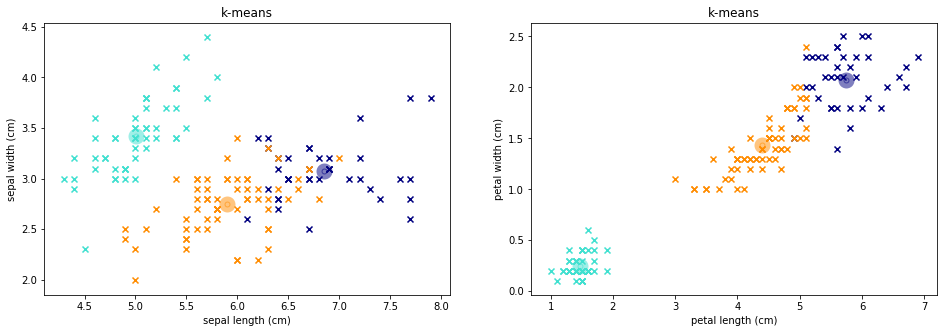
\includegraphics[width=0.9\textwidth]{fig/clusteringKmeans.png}
  \end{figure}
\end{frame}

\begin{frame}{3.1 Mean Shift}
  \begin{itemize}
  \item Cherche les zones de fortes densité en modifiant itérativement la position de \textit{centroïdes}
  \item Des \textit{centroïdes} de rayons $R$ sont aléatoirement initialisés
  \item Ils sont déplacés vers la région de plus haute densité (nombres de points dans le rayon $R$)
  \item On continue jusqu'à maximiser la densité de chaque \textit{centroïde}
  \item Plusieurs \textit{centroïdes} dans une zone: celui avec la plus haute densité est conservé
  \item l'ensemble du dataset est labelisé (plus petite distance)
  \item Le \textit{Mean Shift} détermine le nombre optimal de clusters pour la valeur du rayon choisie (R)
  \end{itemize}
\end{frame}

\begin{frame}{3.1 Clustering: Iris dataset, Mean Shift result}
  \begin{figure}
    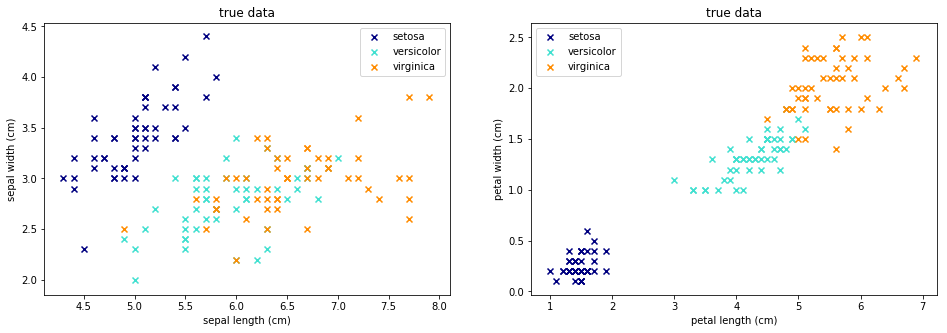
\includegraphics[width=0.9\textwidth]{fig/clusteringTrue.png}
    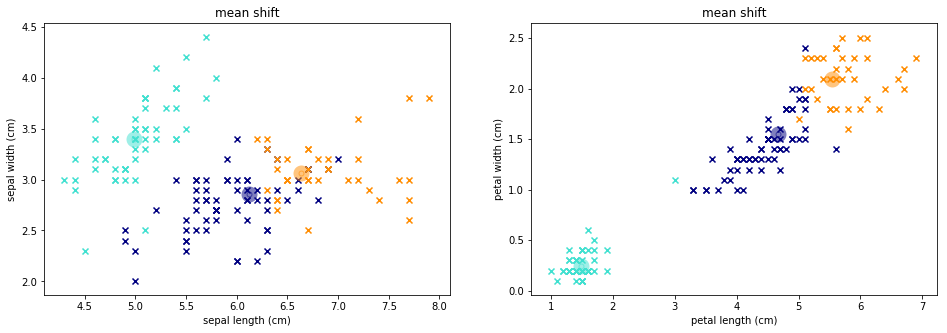
\includegraphics[width=0.9\textwidth]{fig/clusteringMeanShift.png}
  \end{figure}
\end{frame}

\begin{frame}{3.1 Gaussian mixture models}
  \begin{itemize}
  \item \textbf{Hypothèse:} la structure des données est compatible avec un mélange de gaussiènne
  \end{itemize}
  \begin{minipage}{0.48\textwidth}
    \begin{itemize}
    \item On ajuste les paramètres de $N$ gaussiènnes jusqu'à trouver ceux qui \textit{collent} le mieux aux données
    \end{itemize}
  \end{minipage}
  \begin{minipage}{0.48\textwidth}
    \begin{figure}
      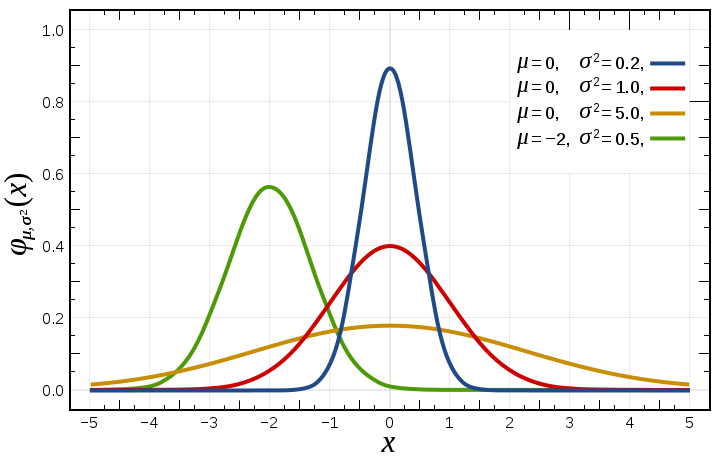
\includegraphics[width=0.8\textwidth]{fig/gaussianFct.png}
    \end{figure}
    \tiny
    \vspace{-0.9cm}
    \begin{center}
      depuis \href{https://en.wikipedia.org/wiki/Gaussian_function}{\color{blue}{Wikipedia}}
    \end{center}
  \end{minipage}
  \begin{itemize}
  \item Algorithme d'ajustement: \textbf{espèrance-maximisation}, on cherche à maximiser la fonction de \textit{log-likelihood} (fonction de vraissemblance)
  \item \textit{Intuitivement:} on cherche les paramètres qui rendent la distribution de données observée la plus probable
  \end{itemize}
\end{frame}

\begin{frame}{3.1 Clustering: Iris dataset, GMM result}
  \begin{figure}
    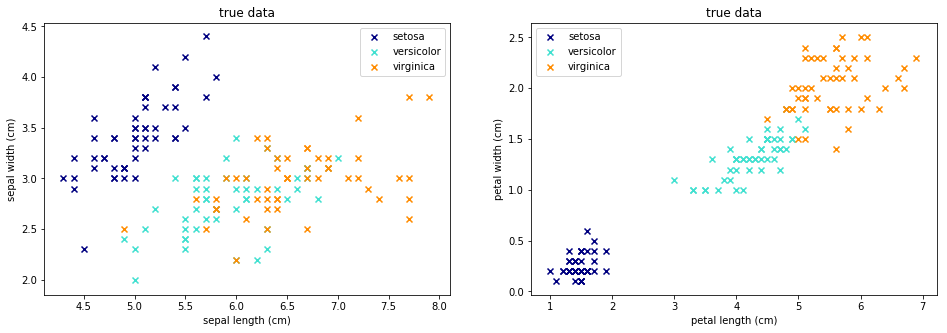
\includegraphics[width=0.9\textwidth]{fig/clusteringTrue.png}
    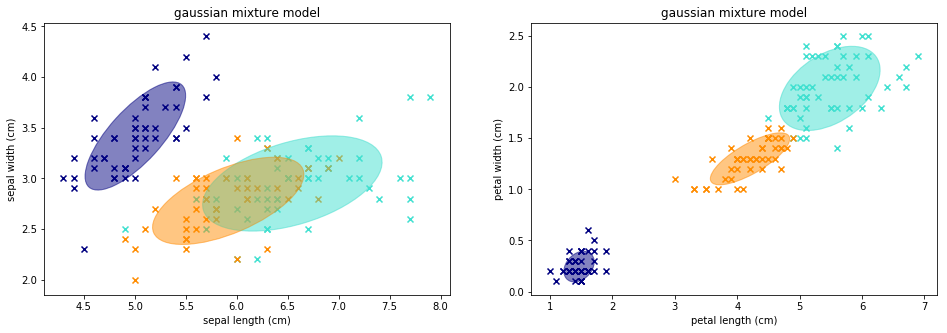
\includegraphics[width=0.9\textwidth]{fig/clusteringGMM.png}
  \end{figure}
\end{frame}

\begin{frame}{3.2 Analyse en composantes principales}
  \begin{itemize}
  \item \textbf{PCA} (\textit{Composants principal analysis}): Algorithme de réduction de dimensions
  \item Transforme un problème à $n$ variables en un problème à $n'$ variables (avec $n' < n$)
  \item Explore les corrélations entre les variables pour les \textit{regrouper} (pondération): \textbf{Pertes d'informations}
  \item Très utile pour:
    \begin{itemize}
      \normalsize
    \item Pre-stage d'un algorithme de clustering (peut améliorer les performances)
    \item Pour faire de la visualisation en 2D de données à plus haute dimension
    \end{itemize}
  \end{itemize}
\end{frame}

\begin{frame}{3.2 Analyse en composantes principales}
  \begin{itemize}
  \item \textbf{Exemple d'utilisation:} digit dataset:
    \begin{itemize}
      \normalsize
    \item 64 variables $\Rightarrow$ 10 pour initialiser le K-means
    \item 64 $\Rightarrow$ 2 pour la visualisation
    \end{itemize}
  \end{itemize}
  \begin{figure}
    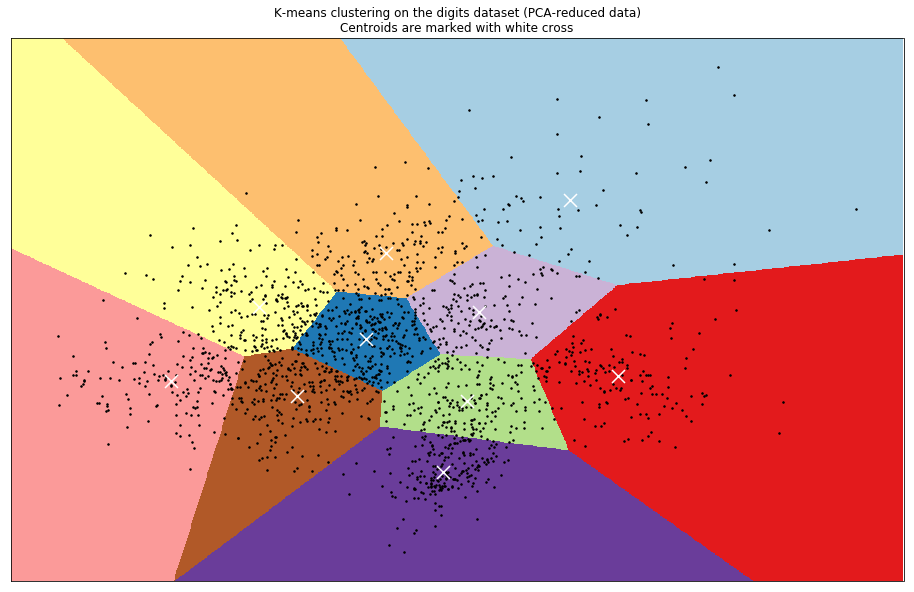
\includegraphics[width=0.8\textwidth]{fig/PCA.png}
  \end{figure}
\end{frame}
